% Options for packages loaded elsewhere
\PassOptionsToPackage{unicode}{hyperref}
\PassOptionsToPackage{hyphens}{url}
%
\documentclass[
]{ctexart}
\usepackage{lmodern}
\usepackage{amsmath}
\usepackage{ifxetex,ifluatex}
\ifnum 0\ifxetex 1\fi\ifluatex 1\fi=0 % if pdftex
  \usepackage[T1]{fontenc}
  \usepackage[utf8]{inputenc}
  \usepackage{textcomp} % provide euro and other symbols
  \usepackage{amssymb}
\else % if luatex or xetex
  \usepackage{unicode-math}
  \defaultfontfeatures{Scale=MatchLowercase}
  \defaultfontfeatures[\rmfamily]{Ligatures=TeX,Scale=1}
\fi
% Use upquote if available, for straight quotes in verbatim environments
\IfFileExists{upquote.sty}{\usepackage{upquote}}{}
\IfFileExists{microtype.sty}{% use microtype if available
  \usepackage[]{microtype}
  \UseMicrotypeSet[protrusion]{basicmath} % disable protrusion for tt fonts
}{}
\makeatletter
\@ifundefined{KOMAClassName}{% if non-KOMA class
  \IfFileExists{parskip.sty}{%
    \usepackage{parskip}
  }{% else
    \setlength{\parindent}{0pt}
    \setlength{\parskip}{6pt plus 2pt minus 1pt}}
}{% if KOMA class
  \KOMAoptions{parskip=half}}
\makeatother
\usepackage{xcolor}
\IfFileExists{xurl.sty}{\usepackage{xurl}}{} % add URL line breaks if available
\IfFileExists{bookmark.sty}{\usepackage{bookmark}}{\usepackage{hyperref}}
\hypersetup{
  pdftitle={Quant\_II\_hwk\_05},
  pdfauthor={吴温泉},
  hidelinks,
  pdfcreator={LaTeX via pandoc}}
\urlstyle{same} % disable monospaced font for URLs
\usepackage[left=2.5cm,right=2cm,top=3cm,bottom=2.5cm]{geometry}
\usepackage{color}
\usepackage{fancyvrb}
\newcommand{\VerbBar}{|}
\newcommand{\VERB}{\Verb[commandchars=\\\{\}]}
\DefineVerbatimEnvironment{Highlighting}{Verbatim}{commandchars=\\\{\}}
% Add ',fontsize=\small' for more characters per line
\usepackage{framed}
\definecolor{shadecolor}{RGB}{248,248,248}
\newenvironment{Shaded}{\begin{snugshade}}{\end{snugshade}}
\newcommand{\AlertTok}[1]{\textcolor[rgb]{0.94,0.16,0.16}{#1}}
\newcommand{\AnnotationTok}[1]{\textcolor[rgb]{0.56,0.35,0.01}{\textbf{\textit{#1}}}}
\newcommand{\AttributeTok}[1]{\textcolor[rgb]{0.77,0.63,0.00}{#1}}
\newcommand{\BaseNTok}[1]{\textcolor[rgb]{0.00,0.00,0.81}{#1}}
\newcommand{\BuiltInTok}[1]{#1}
\newcommand{\CharTok}[1]{\textcolor[rgb]{0.31,0.60,0.02}{#1}}
\newcommand{\CommentTok}[1]{\textcolor[rgb]{0.56,0.35,0.01}{\textit{#1}}}
\newcommand{\CommentVarTok}[1]{\textcolor[rgb]{0.56,0.35,0.01}{\textbf{\textit{#1}}}}
\newcommand{\ConstantTok}[1]{\textcolor[rgb]{0.00,0.00,0.00}{#1}}
\newcommand{\ControlFlowTok}[1]{\textcolor[rgb]{0.13,0.29,0.53}{\textbf{#1}}}
\newcommand{\DataTypeTok}[1]{\textcolor[rgb]{0.13,0.29,0.53}{#1}}
\newcommand{\DecValTok}[1]{\textcolor[rgb]{0.00,0.00,0.81}{#1}}
\newcommand{\DocumentationTok}[1]{\textcolor[rgb]{0.56,0.35,0.01}{\textbf{\textit{#1}}}}
\newcommand{\ErrorTok}[1]{\textcolor[rgb]{0.64,0.00,0.00}{\textbf{#1}}}
\newcommand{\ExtensionTok}[1]{#1}
\newcommand{\FloatTok}[1]{\textcolor[rgb]{0.00,0.00,0.81}{#1}}
\newcommand{\FunctionTok}[1]{\textcolor[rgb]{0.00,0.00,0.00}{#1}}
\newcommand{\ImportTok}[1]{#1}
\newcommand{\InformationTok}[1]{\textcolor[rgb]{0.56,0.35,0.01}{\textbf{\textit{#1}}}}
\newcommand{\KeywordTok}[1]{\textcolor[rgb]{0.13,0.29,0.53}{\textbf{#1}}}
\newcommand{\NormalTok}[1]{#1}
\newcommand{\OperatorTok}[1]{\textcolor[rgb]{0.81,0.36,0.00}{\textbf{#1}}}
\newcommand{\OtherTok}[1]{\textcolor[rgb]{0.56,0.35,0.01}{#1}}
\newcommand{\PreprocessorTok}[1]{\textcolor[rgb]{0.56,0.35,0.01}{\textit{#1}}}
\newcommand{\RegionMarkerTok}[1]{#1}
\newcommand{\SpecialCharTok}[1]{\textcolor[rgb]{0.00,0.00,0.00}{#1}}
\newcommand{\SpecialStringTok}[1]{\textcolor[rgb]{0.31,0.60,0.02}{#1}}
\newcommand{\StringTok}[1]{\textcolor[rgb]{0.31,0.60,0.02}{#1}}
\newcommand{\VariableTok}[1]{\textcolor[rgb]{0.00,0.00,0.00}{#1}}
\newcommand{\VerbatimStringTok}[1]{\textcolor[rgb]{0.31,0.60,0.02}{#1}}
\newcommand{\WarningTok}[1]{\textcolor[rgb]{0.56,0.35,0.01}{\textbf{\textit{#1}}}}
\usepackage{graphicx}
\makeatletter
\def\maxwidth{\ifdim\Gin@nat@width>\linewidth\linewidth\else\Gin@nat@width\fi}
\def\maxheight{\ifdim\Gin@nat@height>\textheight\textheight\else\Gin@nat@height\fi}
\makeatother
% Scale images if necessary, so that they will not overflow the page
% margins by default, and it is still possible to overwrite the defaults
% using explicit options in \includegraphics[width, height, ...]{}
\setkeys{Gin}{width=\maxwidth,height=\maxheight,keepaspectratio}
% Set default figure placement to htbp
\makeatletter
\def\fps@figure{htbp}
\makeatother
\setlength{\emergencystretch}{3em} % prevent overfull lines
\providecommand{\tightlist}{%
  \setlength{\itemsep}{0pt}\setlength{\parskip}{0pt}}
\setcounter{secnumdepth}{5}
\ifluatex
  \usepackage{selnolig}  % disable illegal ligatures
\fi

\title{Quant\_II\_hwk\_05}
\author{吴温泉}
\date{}

\begin{document}
\maketitle

{
\setcounter{tocdepth}{2}
\tableofcontents
}
\hypertarget{ux8ba1ux6570ux56e0ux53d8ux91cfux5206ux6790}{%
\section{计数因变量分析}\label{ux8ba1ux6570ux56e0ux53d8ux91cfux5206ux6790}}

\hypertarget{ux5206ux6790cgss2010-ux6570ux636eux4e2dn35aux95eeux9898ux8bf7ux95eeux4f60ux4e00ux5171ux6350ux732eux8fc7ux591aux5c11ux6b21ux63a2ux8ba8ux6027ux522bux5e74ux9f84ux6536ux5165ux5171ux4ea7ux515aux5458ux5bf9ux4e8eux6350ux732eux6b21ux6570ux7684ux5173ux7cfb}{%
\subsection{分析CGSS2010
数据中n35a问题:``请问你一共捐献过多少次?''探讨性别、年龄、收入、共产党员对于捐献次数的关系。}\label{ux5206ux6790cgss2010-ux6570ux636eux4e2dn35aux95eeux9898ux8bf7ux95eeux4f60ux4e00ux5171ux6350ux732eux8fc7ux591aux5c11ux6b21ux63a2ux8ba8ux6027ux522bux5e74ux9f84ux6536ux5165ux5171ux4ea7ux515aux5458ux5bf9ux4e8eux6350ux732eux6b21ux6570ux7684ux5173ux7cfb}}

\begin{Shaded}
\begin{Highlighting}[]
\NormalTok{dat }\OtherTok{\textless{}{-}} \FunctionTok{read\_dta}\NormalTok{(}\StringTok{"cgss2010\_14.dta"}\NormalTok{)}

\CommentTok{\# summary(dat)}
\NormalTok{male }\OtherTok{\textless{}{-}} \FunctionTok{ifelse}\NormalTok{(dat}\SpecialCharTok{$}\NormalTok{a2}\SpecialCharTok{==}\DecValTok{1}\NormalTok{, }\DecValTok{1}\NormalTok{,}
    \FunctionTok{ifelse}\NormalTok{(dat}\SpecialCharTok{$}\NormalTok{a2}\SpecialCharTok{==}\DecValTok{2}\NormalTok{, }\DecValTok{0}\NormalTok{, }\ConstantTok{NA}\NormalTok{)) }\CommentTok{\# gender}
\NormalTok{a3a }\OtherTok{\textless{}{-}} \FunctionTok{ifelse}\NormalTok{(dat}\SpecialCharTok{$}\NormalTok{a3a }\SpecialCharTok{\textless{}} \DecValTok{17}\NormalTok{, }\ConstantTok{NA}\NormalTok{, dat}\SpecialCharTok{$}\NormalTok{a3a)  }\CommentTok{\# age}
\NormalTok{age }\OtherTok{\textless{}{-}} \DecValTok{2010}\SpecialCharTok{{-}}\NormalTok{a3a}
\NormalTok{a62 }\OtherTok{\textless{}{-}} \FunctionTok{ifelse}\NormalTok{(dat}\SpecialCharTok{$}\NormalTok{a62 }\SpecialCharTok{\textgreater{}} \DecValTok{9999996}\NormalTok{, }\ConstantTok{NA}\NormalTok{, dat}\SpecialCharTok{$}\NormalTok{a62) }\CommentTok{\# income}
\NormalTok{ccpmember }\OtherTok{\textless{}{-}} \FunctionTok{ifelse}\NormalTok{(dat}\SpecialCharTok{$}\NormalTok{a10 }\SpecialCharTok{==} \DecValTok{1}\NormalTok{, }\DecValTok{1}\NormalTok{, }\DecValTok{0}\NormalTok{) }\CommentTok{\# member}
\NormalTok{probs }\OtherTok{\textless{}{-}} \FunctionTok{c}\NormalTok{(}\DecValTok{0}\NormalTok{, }\FloatTok{0.07}\NormalTok{, }\FloatTok{0.25}\NormalTok{, }\FloatTok{0.5}\NormalTok{, }\FloatTok{0.75}\NormalTok{, }\FloatTok{0.93}\NormalTok{, }\DecValTok{1}\NormalTok{)}
\NormalTok{kpts }\OtherTok{\textless{}{-}} \FunctionTok{quantile}\NormalTok{(a62, }\AttributeTok{prob=}\NormalTok{probs, }\AttributeTok{na.rm=}\ConstantTok{TRUE}\NormalTok{)}
\NormalTok{hinc }\OtherTok{\textless{}{-}} \FunctionTok{as.numeric}\NormalTok{(}\FunctionTok{cut}\NormalTok{(a62, }\AttributeTok{breaks=}\NormalTok{kpts, }\AttributeTok{labels =} \DecValTok{1}\SpecialCharTok{:}\DecValTok{6}\NormalTok{, }\AttributeTok{right=}\ConstantTok{TRUE}\NormalTok{))}
\NormalTok{kpts2 }\OtherTok{\textless{}{-}} \FunctionTok{quantile}\NormalTok{(a62, }\AttributeTok{prob=}\FunctionTok{c}\NormalTok{(}\DecValTok{0}\NormalTok{,}\DecValTok{1}\SpecialCharTok{/}\DecValTok{6}\NormalTok{,}\DecValTok{2}\SpecialCharTok{/}\DecValTok{6}\NormalTok{,}\DecValTok{3}\SpecialCharTok{/}\DecValTok{6}\NormalTok{,}\DecValTok{4}\SpecialCharTok{/}\DecValTok{6}\NormalTok{,}\DecValTok{5}\SpecialCharTok{/}\DecValTok{6}\NormalTok{,}\DecValTok{1}\NormalTok{), }\AttributeTok{na.rm=}\ConstantTok{TRUE}\NormalTok{)}
\NormalTok{hinc2 }\OtherTok{\textless{}{-}} \FunctionTok{as.numeric}\NormalTok{(}\FunctionTok{cut}\NormalTok{(a62, }\AttributeTok{breaks=}\NormalTok{kpts2, }\AttributeTok{labels =} \DecValTok{1}\SpecialCharTok{:}\DecValTok{6}\NormalTok{, }\AttributeTok{right=}\ConstantTok{TRUE}\NormalTok{))}
\NormalTok{loghinc }\OtherTok{\textless{}{-}} \FunctionTok{log}\NormalTok{(a62}\SpecialCharTok{+}\DecValTok{1}\NormalTok{)}

\NormalTok{n35a }\OtherTok{\textless{}{-}} \FunctionTok{ifelse}\NormalTok{(dat}\SpecialCharTok{$}\NormalTok{n35a}\SpecialCharTok{\textless{}}\DecValTok{0}\NormalTok{, }\DecValTok{0}\NormalTok{, dat}\SpecialCharTok{$}\NormalTok{n35a)}

\CommentTok{\# dat1 \textless{}{-} cbind.data.frame("contribution"=factor(n35a), male, age, loghinc, ccpmember)}
\NormalTok{dat1 }\OtherTok{\textless{}{-}} \FunctionTok{cbind.data.frame}\NormalTok{(}\StringTok{"contribution"}\OtherTok{=}\NormalTok{n35a, male, age, loghinc, ccpmember)}
\NormalTok{dat2 }\OtherTok{\textless{}{-}} \FunctionTok{na.exclude}\NormalTok{(dat1)}
\end{Highlighting}
\end{Shaded}

\hypertarget{ux4f7fux7528poisson-ux5206ux6790ux6027ux522bux5e74ux9f84ux6536ux5165ux5171ux4ea7ux515aux5458ux81eaux53d8ux91cfux5bf9ux6350ux732eux6b21ux6570ux56e0ux53d8ux91cfux7684ux5173ux7cfbux521dux6b65ux4f7fux7528ux7cfbux6570ux7684ux6b63ux8d1fux5173ux7cfbux89e3ux8bfbux56e0ux53d8ux91cfux548cux81eaux53d8ux91cfux7684ux5173ux7cfbux5e76ux8bf4ux660e-peudo-r2-ux548cux4f3cux7136ux503cux68c0ux9a8cux7684ux7ed3ux679c}{%
\subsection{使用poisson
分析性别、年龄、收入、共产党员(自变量)对捐献次数(因变量)的关系,初步使用系数的正负关系解读因变量和自变量的关系,并说明
Peudo-R2
和似然值检验的结果。}\label{ux4f7fux7528poisson-ux5206ux6790ux6027ux522bux5e74ux9f84ux6536ux5165ux5171ux4ea7ux515aux5458ux81eaux53d8ux91cfux5bf9ux6350ux732eux6b21ux6570ux56e0ux53d8ux91cfux7684ux5173ux7cfbux521dux6b65ux4f7fux7528ux7cfbux6570ux7684ux6b63ux8d1fux5173ux7cfbux89e3ux8bfbux56e0ux53d8ux91cfux548cux81eaux53d8ux91cfux7684ux5173ux7cfbux5e76ux8bf4ux660e-peudo-r2-ux548cux4f3cux7136ux503cux68c0ux9a8cux7684ux7ed3ux679c}}

\begin{Shaded}
\begin{Highlighting}[]
\NormalTok{M1 }\OtherTok{\textless{}{-}} \FunctionTok{glm}\NormalTok{(contribution }\SpecialCharTok{\textasciitilde{}}\NormalTok{ male }\SpecialCharTok{+}\NormalTok{ age }\SpecialCharTok{+}\NormalTok{ loghinc }\SpecialCharTok{+}\NormalTok{ ccpmember, }\AttributeTok{data=}\NormalTok{dat1, }\AttributeTok{family=}\FunctionTok{poisson}\NormalTok{(}\AttributeTok{link=}\StringTok{"log"}\NormalTok{))}
\FunctionTok{summary}\NormalTok{(M1)}
\end{Highlighting}
\end{Shaded}

\begin{verbatim}
## 
## Call:
## glm(formula = contribution ~ male + age + loghinc + ccpmember, 
##     family = poisson(link = "log"), data = dat1)
## 
## Deviance Residuals: 
##    Min      1Q  Median      3Q     Max  
## -4.034  -2.371  -1.774  -0.673  60.068  
## 
## Coefficients:
##              Estimate Std. Error z value Pr(>|z|)    
## (Intercept)  1.748968   0.143660  12.174  < 2e-16 ***
## male        -0.074535   0.030916  -2.411 0.015913 *  
## age          0.010596   0.001012  10.469  < 2e-16 ***
## loghinc     -0.043300   0.012294  -3.522 0.000428 ***
## ccpmember   -0.157643   0.054592  -2.888 0.003881 ** 
## ---
## Signif. codes:  0 '***' 0.001 '**' 0.01 '*' 0.05 '.' 0.1 ' ' 1
## 
## (Dispersion parameter for poisson family taken to be 1)
## 
##     Null deviance: 12263  on 789  degrees of freedom
## Residual deviance: 12099  on 785  degrees of freedom
##   (10993 observations deleted due to missingness)
## AIC: 14258
## 
## Number of Fisher Scoring iterations: 7
\end{verbatim}

\begin{Shaded}
\begin{Highlighting}[]
\CommentTok{\# pseudo R2}
\NormalTok{M0 }\OtherTok{\textless{}{-}} \FunctionTok{update}\NormalTok{(M1, .}\SpecialCharTok{\textasciitilde{}}\DecValTok{1}\NormalTok{)}
\NormalTok{devNull }\OtherTok{\textless{}{-}} \FunctionTok{deviance}\NormalTok{(M0)}
\NormalTok{dev }\OtherTok{\textless{}{-}} \FunctionTok{deviance}\NormalTok{(M1)}
\NormalTok{pR2 }\OtherTok{\textless{}{-}}\NormalTok{ (devNull }\SpecialCharTok{{-}}\NormalTok{ dev) }\SpecialCharTok{/}\NormalTok{ devNull}
\NormalTok{pR2}
\end{Highlighting}
\end{Shaded}

\begin{verbatim}
## [1] 0.04932302
\end{verbatim}

\begin{Shaded}
\begin{Highlighting}[]
\CommentTok{\# likelihood ratio test}
\NormalTok{LR }\OtherTok{\textless{}{-}}\NormalTok{ devNull }\SpecialCharTok{{-}}\NormalTok{ dev}
\NormalTok{k }\OtherTok{\textless{}{-}} \FunctionTok{length}\NormalTok{(}\FunctionTok{coef}\NormalTok{(M1))}
\NormalTok{prob }\OtherTok{\textless{}{-}} \FunctionTok{pchisq}\NormalTok{(LR, }\AttributeTok{df=}\NormalTok{k}\DecValTok{{-}1}\NormalTok{, }\AttributeTok{lower.tail =} \ConstantTok{FALSE}\NormalTok{)}
\NormalTok{prob}
\end{Highlighting}
\end{Shaded}

\begin{verbatim}
## [1] 1.567043e-134
\end{verbatim}

Peudo-R2:有自变量的模型较没有自变数的模型可以解释的偏差比为4.9\%
似然值检验显著,有自变量的模型较没有自变数的模型可以解释y更多的偏差,拟合优度(goodness
of fit) 显著性改善。 \#\# 使用事件发生率比(incidence rate ratio)
解释因变量和自变量的关系。

\begin{Shaded}
\begin{Highlighting}[]
\CommentTok{\# irr, incidence rate ratio}
\NormalTok{IRR }\OtherTok{\textless{}{-}} \ControlFlowTok{function}\NormalTok{(fit, newdata)\{}
\NormalTok{    IR }\OtherTok{\textless{}{-}} \FunctionTok{predict}\NormalTok{(fit, newdata, }\AttributeTok{type =} \StringTok{"response"}\NormalTok{) }\CommentTok{\#lambdas}
\NormalTok{    IRR }\OtherTok{\textless{}{-}}\NormalTok{ IR[}\DecValTok{2}\NormalTok{]}\SpecialCharTok{/}\NormalTok{IR[}\DecValTok{1}\NormalTok{]}
    \FunctionTok{return}\NormalTok{(IRR)}
\NormalTok{\}}

\FunctionTok{IRR}\NormalTok{(M1, dat1)}
\end{Highlighting}
\end{Shaded}

\begin{verbatim}
##        2 
## 1.032884
\end{verbatim}

\hypertarget{ux6bd4ux8f8330-ux5c81ux6536ux5165ux4e3aux5747ux503cux7684ux5171ux4ea7ux515aux515aux5458ux7537ux6027ux548cux5973ux6027ux4e4bux95f4ux5728ux6350ux732eux6b21ux6570ux7684ux5deeux5f02}{%
\subsection{比较30
岁、收入为均值的共产党党员男性和女性之间在捐献次数的差异。}\label{ux6bd4ux8f8330-ux5c81ux6536ux5165ux4e3aux5747ux503cux7684ux5171ux4ea7ux515aux515aux5458ux7537ux6027ux548cux5973ux6027ux4e4bux95f4ux5728ux6350ux732eux6b21ux6570ux7684ux5deeux5f02}}

\begin{Shaded}
\begin{Highlighting}[]
\CommentTok{\# predictive difference between gender}
\NormalTok{newX }\OtherTok{\textless{}{-}} \FunctionTok{with}\NormalTok{(dat2, }\FunctionTok{cbind.data.frame}\NormalTok{(}\AttributeTok{male =} \FunctionTok{c}\NormalTok{(}\DecValTok{0}\NormalTok{,}\DecValTok{1}\NormalTok{), }\AttributeTok{age =} \DecValTok{30}\NormalTok{, }\AttributeTok{loghinc =} \FunctionTok{mean}\NormalTok{(loghinc), }
                                    \AttributeTok{ccpmember =} \DecValTok{1}\NormalTok{))}
\NormalTok{phat }\OtherTok{\textless{}{-}} \FunctionTok{predict}\NormalTok{(M1, }\AttributeTok{newdata=}\NormalTok{newX, }\AttributeTok{type =} \StringTok{"terms"}\NormalTok{)}
\NormalTok{phat[}\DecValTok{2}\NormalTok{,] }\SpecialCharTok{{-}}\NormalTok{ phat[}\DecValTok{1}\NormalTok{,]}
\end{Highlighting}
\end{Shaded}

\begin{verbatim}
##        male         age     loghinc   ccpmember 
## -0.07453545  0.00000000  0.00000000  0.00000000
\end{verbatim}

比较除了性别以外相同的两个人,男性比女性少7 \% 的概率认为社会是公正的。

\hypertarget{ux4f7fux7528ux7ed8ux56feux7684ux65b9ux5f0fux5448ux73b0ux6709ux81eaux53d8ux91cfux7684ux6a21ux578bux548cux6ca1ux6709ux81eaux53d8ux91cfux7684ux6a21ux578bux5bf9ux4e8eux9884ux6d4bux6350ux732eux6b21ux6570ux6982ux7387ux7684ux5deeux522b}{%
\subsection{使用绘图的方式,呈现有自变量的模型和没有自变量的模型对于预测捐献次数概率的差别。}\label{ux4f7fux7528ux7ed8ux56feux7684ux65b9ux5f0fux5448ux73b0ux6709ux81eaux53d8ux91cfux7684ux6a21ux578bux548cux6ca1ux6709ux81eaux53d8ux91cfux7684ux6a21ux578bux5bf9ux4e8eux9884ux6d4bux6350ux732eux6b21ux6570ux6982ux7387ux7684ux5deeux522b}}

\begin{Shaded}
\begin{Highlighting}[]
\CommentTok{\# newX \textless{}{-} dat2}
\NormalTok{newX }\OtherTok{\textless{}{-}} \FunctionTok{with}\NormalTok{(dat2, }\FunctionTok{cbind.data.frame}\NormalTok{(}\AttributeTok{male =} \FunctionTok{mean}\NormalTok{(male), }\AttributeTok{age =} \FunctionTok{mean}\NormalTok{(age),  }\AttributeTok{loghinc =} \FunctionTok{mean}\NormalTok{(loghinc), }\AttributeTok{ccpmember =} \FunctionTok{mean}\NormalTok{(ccpmember)))}


\NormalTok{numContri }\OtherTok{\textless{}{-}} \FunctionTok{seq}\NormalTok{(}\DecValTok{0}\NormalTok{, }\FunctionTok{max}\NormalTok{(dat2}\SpecialCharTok{$}\NormalTok{contribution))}
\NormalTok{K }\OtherTok{\textless{}{-}} \FunctionTok{length}\NormalTok{(numContri)}
\NormalTok{phatN }\OtherTok{\textless{}{-}}\NormalTok{ phatS }\OtherTok{\textless{}{-}} \FunctionTok{rep}\NormalTok{(}\ConstantTok{NA}\NormalTok{, K)}
\ControlFlowTok{for}\NormalTok{(i }\ControlFlowTok{in} \DecValTok{1}\SpecialCharTok{:}\NormalTok{K)\{}
\NormalTok{    lamS }\OtherTok{\textless{}{-}} \FunctionTok{predict}\NormalTok{(M1, }\AttributeTok{newdata=}\NormalTok{newX, }\AttributeTok{type=}\StringTok{"response"}\NormalTok{)}
\NormalTok{    phatS[i] }\OtherTok{\textless{}{-}} \FunctionTok{dpois}\NormalTok{(numContri[i], }\AttributeTok{lambda=}\NormalTok{lamS)}
\NormalTok{    lamN }\OtherTok{\textless{}{-}} \FunctionTok{predict}\NormalTok{(M0, }\AttributeTok{newdata=}\NormalTok{newX, }\AttributeTok{type=}\StringTok{"response"}\NormalTok{)}
\NormalTok{    phatN[i] }\OtherTok{\textless{}{-}} \FunctionTok{dpois}\NormalTok{(numContri[i], }\AttributeTok{lambda=}\NormalTok{lamN)}
\NormalTok{\}}

\NormalTok{tabContri }\OtherTok{\textless{}{-}} \FunctionTok{table}\NormalTok{(dat1}\SpecialCharTok{$}\NormalTok{contribution)}
\NormalTok{pObserved }\OtherTok{\textless{}{-}}\NormalTok{ tabContri }\SpecialCharTok{/} \FunctionTok{sum}\NormalTok{(tabContri)}
\NormalTok{xObserved }\OtherTok{\textless{}{-}} \FunctionTok{names}\NormalTok{(pObserved)}


\FunctionTok{plot}\NormalTok{(}\DecValTok{0}\NormalTok{, }\DecValTok{0}\NormalTok{, }\AttributeTok{xlim =}\FunctionTok{c}\NormalTok{(}\DecValTok{0}\NormalTok{, K), }\AttributeTok{ylim=}\FunctionTok{c}\NormalTok{(}\DecValTok{0}\NormalTok{, }\FloatTok{0.4}\NormalTok{), }\AttributeTok{type=}\StringTok{"n"}\NormalTok{, }\AttributeTok{axes=}\ConstantTok{FALSE}\NormalTok{, }\AttributeTok{frame.plot=}\ConstantTok{TRUE}\NormalTok{,}
    \AttributeTok{ylab=}\StringTok{"Probability of count"}\NormalTok{, }\AttributeTok{xlab=}\StringTok{"Number of contributions"}\NormalTok{)}
\FunctionTok{lines}\NormalTok{(}\AttributeTok{x =}\NormalTok{ xObserved, }\AttributeTok{y =}\NormalTok{ pObserved)}
\CommentTok{\#segments(x0=as.numeric(xObserved), y0=0, x1=as.numeric(xObserved), y1=pObserved)}
\FunctionTok{lines}\NormalTok{(}\AttributeTok{x =} \DecValTok{1}\SpecialCharTok{:}\NormalTok{K, }\AttributeTok{y =}\NormalTok{ phatS, }\AttributeTok{col=}\DecValTok{2}\NormalTok{)}
\FunctionTok{lines}\NormalTok{(}\AttributeTok{x =} \DecValTok{1}\SpecialCharTok{:}\NormalTok{K, }\AttributeTok{y =}\NormalTok{ phatN, }\AttributeTok{col=}\DecValTok{3}\NormalTok{)}
\FunctionTok{legend}\NormalTok{(}\StringTok{"topright"}\NormalTok{, }\AttributeTok{col=}\DecValTok{1}\SpecialCharTok{:}\DecValTok{3}\NormalTok{, }\AttributeTok{lty=}\DecValTok{1}\NormalTok{, }\AttributeTok{legend=}\FunctionTok{c}\NormalTok{(}\StringTok{"Observed"}\NormalTok{, }\StringTok{"Saturated model"}\NormalTok{, }\StringTok{"Null model"}\NormalTok{))}
\FunctionTok{axis}\NormalTok{(}\DecValTok{2}\NormalTok{)}
\FunctionTok{axis}\NormalTok{(}\DecValTok{1}\NormalTok{)}
\end{Highlighting}
\end{Shaded}

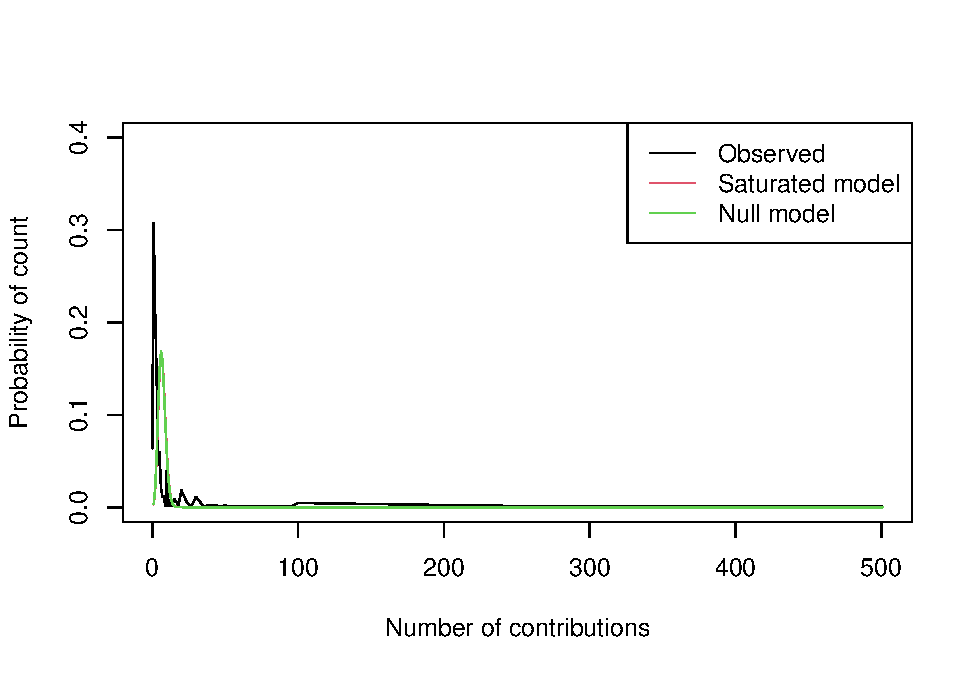
\includegraphics{hwk05_files/figure-latex/unnamed-chunk-6-1.pdf}

\hypertarget{ux4f7fux7528ux7ed8ux56feux7684ux65b9ux5f0fux5448ux73b0ux515aux5458ux548cux975eux515aux5458ux768430-ux5c81ux7537ux6027ux4ed6ux5728ux4e0dux540cux6536ux5165ux6350ux732e5-ux6b21ux7684ux6982ux7387ux5deeux522bux4f60ux89c2ux5bdfux5230ux4ec0ux4e48ux73b0ux8c61}{%
\subsection{使用绘图的方式,呈现党员和非党员的30
岁男性,他在不同收入捐献5
次的概率差别。你观察到什么现象。}\label{ux4f7fux7528ux7ed8ux56feux7684ux65b9ux5f0fux5448ux73b0ux515aux5458ux548cux975eux515aux5458ux768430-ux5c81ux7537ux6027ux4ed6ux5728ux4e0dux540cux6536ux5165ux6350ux732e5-ux6b21ux7684ux6982ux7387ux5deeux522bux4f60ux89c2ux5bdfux5230ux4ec0ux4e48ux73b0ux8c61}}

\begin{Shaded}
\begin{Highlighting}[]
\NormalTok{rangeInc }\OtherTok{\textless{}{-}} \FunctionTok{with}\NormalTok{(dat2, }\FunctionTok{range}\NormalTok{(loghinc))}
\NormalTok{incFake }\OtherTok{\textless{}{-}} \FunctionTok{seq}\NormalTok{(rangeInc[}\DecValTok{1}\NormalTok{],rangeInc[}\DecValTok{2}\NormalTok{],}\AttributeTok{length=}\DecValTok{1000}\NormalTok{)}
\NormalTok{newXY }\OtherTok{\textless{}{-}} \FunctionTok{with}\NormalTok{(dat2, }\FunctionTok{cbind.data.frame}\NormalTok{(}\AttributeTok{male =} \DecValTok{1}\NormalTok{, }\AttributeTok{age =} \DecValTok{30}\NormalTok{, }\AttributeTok{ccpmember =} \DecValTok{1}\NormalTok{, }\AttributeTok{loghinc =}\NormalTok{ incFake))}
\NormalTok{newXN }\OtherTok{\textless{}{-}} \FunctionTok{with}\NormalTok{(dat2, }\FunctionTok{cbind.data.frame}\NormalTok{(}\AttributeTok{male =} \DecValTok{1}\NormalTok{, }\AttributeTok{age =} \DecValTok{30}\NormalTok{, }\AttributeTok{ccpmember =} \DecValTok{0}\NormalTok{, }\AttributeTok{loghinc =}\NormalTok{ incFake))}
\NormalTok{lambdaY }\OtherTok{\textless{}{-}} \FunctionTok{predict}\NormalTok{(M1, }\AttributeTok{newdata=}\NormalTok{newXY, }\AttributeTok{type =} \StringTok{"response"}\NormalTok{)}
\NormalTok{lambdaN }\OtherTok{\textless{}{-}} \FunctionTok{predict}\NormalTok{(M1, }\AttributeTok{newdata=}\NormalTok{newXN, }\AttributeTok{type =} \StringTok{"response"}\NormalTok{)}

\NormalTok{N }\OtherTok{\textless{}{-}} \DecValTok{5} \CommentTok{\# publish 2 papers}
\NormalTok{phatY }\OtherTok{\textless{}{-}} \FunctionTok{dpois}\NormalTok{(N, lambdaY) }\CommentTok{\# compute predictive probability given N = 2, and lambda predicted from the model}
\NormalTok{phatN }\OtherTok{\textless{}{-}} \FunctionTok{dpois}\NormalTok{(N, lambdaN)}

\FunctionTok{par}\NormalTok{(}\AttributeTok{mar=}\FunctionTok{c}\NormalTok{(}\DecValTok{3}\NormalTok{,}\DecValTok{3}\NormalTok{,}\DecValTok{1}\NormalTok{,}\DecValTok{1}\NormalTok{), }\AttributeTok{mgp=}\FunctionTok{c}\NormalTok{(}\DecValTok{2}\NormalTok{,}\FloatTok{0.5}\NormalTok{,}\DecValTok{0}\NormalTok{), }\AttributeTok{tcl=}\SpecialCharTok{{-}}\FloatTok{0.2}\NormalTok{)}
\FunctionTok{plot}\NormalTok{(}\AttributeTok{x=}\NormalTok{incFake, }\AttributeTok{y=}\NormalTok{phatY, }\AttributeTok{type=}\StringTok{"l"}\NormalTok{, }\AttributeTok{xlim=}\NormalTok{rangeInc, }\AttributeTok{ylim=}\FunctionTok{c}\NormalTok{(}\DecValTok{0}\NormalTok{,}\FloatTok{0.5}\NormalTok{),}
    \AttributeTok{xlab =} \StringTok{"Loginc"}\NormalTok{, }\AttributeTok{ylab =} \StringTok{"Pr(contribution = 5)"}\NormalTok{)}
\FunctionTok{lines}\NormalTok{(}\AttributeTok{x =}\NormalTok{ incFake, }\AttributeTok{y=}\NormalTok{phatN, }\AttributeTok{col=}\DecValTok{2}\NormalTok{)}
\FunctionTok{text}\NormalTok{(}\AttributeTok{x =}\NormalTok{ incFake[}\DecValTok{500}\NormalTok{], }\AttributeTok{y =}\NormalTok{ phatY[}\DecValTok{500}\NormalTok{], }\StringTok{"CCP Member"}\NormalTok{, }\AttributeTok{adj=}\DecValTok{0}\NormalTok{)}
\FunctionTok{text}\NormalTok{(}\AttributeTok{x =}\NormalTok{ incFake[}\DecValTok{500}\NormalTok{], }\AttributeTok{y =}\NormalTok{ phatN[}\DecValTok{500}\NormalTok{], }\StringTok{"Not CCP Member"}\NormalTok{, }\AttributeTok{adj=}\DecValTok{1}\NormalTok{, }\AttributeTok{col=}\DecValTok{2}\NormalTok{)}
\end{Highlighting}
\end{Shaded}

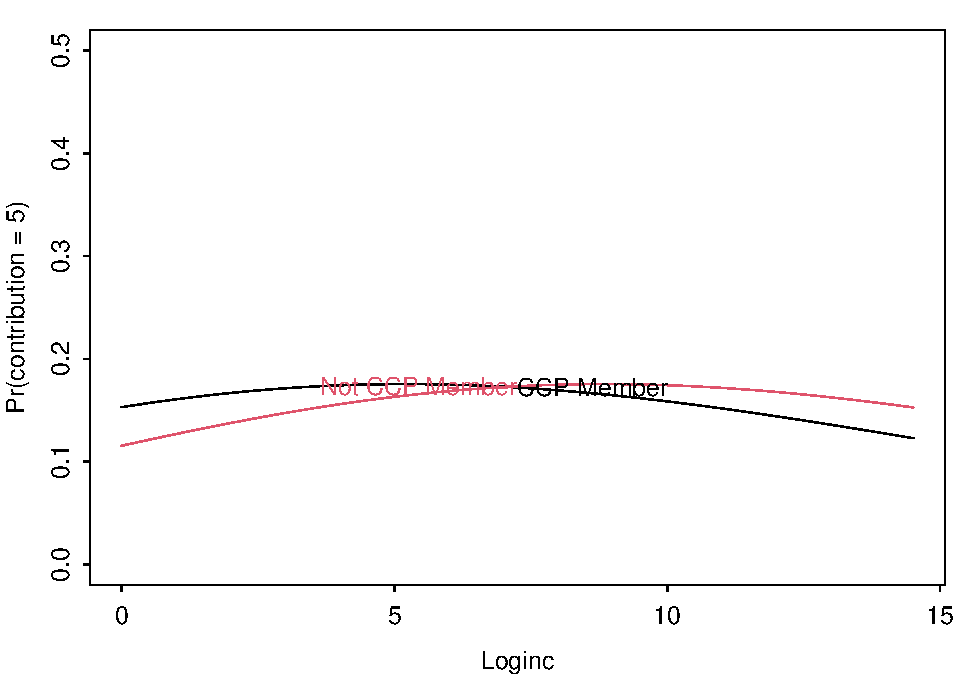
\includegraphics{hwk05_files/figure-latex/unnamed-chunk-7-1.pdf}

\begin{Shaded}
\begin{Highlighting}[]
\CommentTok{\#legend("topright", lty=1, col=c(1,2), legend = c("Female", "Male"))}
\CommentTok{\# legend(locator(1), lty=1, col=c(1,2), legend = c("CCP Member", "Not CCP Member"))}
\end{Highlighting}
\end{Shaded}

可以发现,比较除了政治面貌以外相同的两个人,在收入较低时,党员比非党员捐献五次的几率更大;随着收入的增加,非党员捐献五次的几率逐渐超过党员。

\hypertarget{ux4f7fux7528ux8d1fux4e8cux9879ux56deux5f52ux91cdux65b0ux68c0ux9a8cux4e0aux8ff0ux5173ux7cfbux4f60ux8ba4ux4e3apoisson-ux548cux8d1fux4e8cux9879ux56deux5f52ux90a3ux4e2aux6bd4ux8f83ux5408-ux9002ux4f60ux7684ux4e3bux5f20ux6839ux636eux662fux4ec0ux4e48ux63d0ux793aalphaux68c0ux9a8c}{%
\subsection{\texorpdfstring{使用负二项回归重新检验上述关系,你认为poisson
和负二项回归那个比较合
适?你的主张根据是什么?(提示:\(\alpha\)检验)}{使用负二项回归重新检验上述关系,你认为poisson 和负二项回归那个比较合 适?你的主张根据是什么?(提示:\textbackslash alpha检验)}}\label{ux4f7fux7528ux8d1fux4e8cux9879ux56deux5f52ux91cdux65b0ux68c0ux9a8cux4e0aux8ff0ux5173ux7cfbux4f60ux8ba4ux4e3apoisson-ux548cux8d1fux4e8cux9879ux56deux5f52ux90a3ux4e2aux6bd4ux8f83ux5408-ux9002ux4f60ux7684ux4e3bux5f20ux6839ux636eux662fux4ec0ux4e48ux63d0ux793aalphaux68c0ux9a8c}}

\begin{Shaded}
\begin{Highlighting}[]
\CommentTok{\# negative binomial}
\FunctionTok{library}\NormalTok{(MASS)}
\end{Highlighting}
\end{Shaded}

\begin{verbatim}
## Warning: package 'MASS' was built under R version 4.0.3
\end{verbatim}

\begin{verbatim}
## 
## Attaching package: 'MASS'
\end{verbatim}

\begin{verbatim}
## The following object is masked from 'package:dplyr':
## 
##     select
\end{verbatim}

\begin{Shaded}
\begin{Highlighting}[]
\NormalTok{M3 }\OtherTok{\textless{}{-}} \FunctionTok{glm.nb}\NormalTok{(contribution }\SpecialCharTok{\textasciitilde{}}\NormalTok{ male }\SpecialCharTok{+}\NormalTok{ age }\SpecialCharTok{+}\NormalTok{ ccpmember }\SpecialCharTok{+}\NormalTok{ loghinc, }\AttributeTok{data=}\NormalTok{dat1)}
\FunctionTok{summary}\NormalTok{(M3)}
\end{Highlighting}
\end{Shaded}

\begin{verbatim}
## 
## Call:
## glm.nb(formula = contribution ~ male + age + ccpmember + loghinc, 
##     data = dat1, init.theta = 0.644737165, link = log)
## 
## Deviance Residuals: 
##     Min       1Q   Median       3Q      Max  
## -1.8368  -0.9584  -0.6537  -0.2605  10.4023  
## 
## Coefficients:
##              Estimate Std. Error z value Pr(>|z|)    
## (Intercept)  1.863680   0.475720   3.918 8.94e-05 ***
## male        -0.015511   0.097240  -0.160  0.87326    
## age          0.009649   0.003272   2.949  0.00319 ** 
## ccpmember   -0.126392   0.163313  -0.774  0.43898    
## loghinc     -0.052712   0.041059  -1.284  0.19921    
## ---
## Signif. codes:  0 '***' 0.001 '**' 0.01 '*' 0.05 '.' 0.1 ' ' 1
## 
## (Dispersion parameter for Negative Binomial(0.6447) family taken to be 1)
## 
##     Null deviance: 868.37  on 789  degrees of freedom
## Residual deviance: 853.81  on 785  degrees of freedom
##   (10993 observations deleted due to missingness)
## AIC: 4408.9
## 
## Number of Fisher Scoring iterations: 1
## 
## 
##               Theta:  0.6447 
##           Std. Err.:  0.0324 
## 
##  2 x log-likelihood:  -4396.8550
\end{verbatim}

\begin{Shaded}
\begin{Highlighting}[]
\CommentTok{\# alpha test}
\NormalTok{G2 }\OtherTok{\textless{}{-}} \DecValTok{2}\SpecialCharTok{*}\NormalTok{(}\FunctionTok{logLik}\NormalTok{(M3) }\SpecialCharTok{{-}} \FunctionTok{logLik}\NormalTok{(M1))}
\FunctionTok{pchisq}\NormalTok{(G2, }\AttributeTok{df=}\DecValTok{1}\NormalTok{, }\AttributeTok{lower.tail=}\ConstantTok{FALSE}\NormalTok{)}
\end{Highlighting}
\end{Shaded}

\begin{verbatim}
## 'log Lik.' 0 (df=6)
\end{verbatim}

\begin{Shaded}
\begin{Highlighting}[]
\CommentTok{\# H0: Negbin is the same as Poisson (alpha=0)}
\end{Highlighting}
\end{Shaded}

G2显著,因此拒绝零假设,负二项回归合适

\hypertarget{ux4f7fux7528ux96f6ux81a8ux80c0ux8ba1ux6570ux56deux5f52ux91cdux65b0ux68c0ux9a8cux4e0aux8ff0ux5173ux7cfbux540cux65f6ux8003ux8651ux96f6ux81a8ux80c0poisson-ux548cux8d1fux4e8cux9879ux56deux5f52}{%
\subsection{使用零膨胀计数回归重新检验上述关系(同时考虑零膨胀poisson
和负二项回归)。}\label{ux4f7fux7528ux96f6ux81a8ux80c0ux8ba1ux6570ux56deux5f52ux91cdux65b0ux68c0ux9a8cux4e0aux8ff0ux5173ux7cfbux540cux65f6ux8003ux8651ux96f6ux81a8ux80c0poisson-ux548cux8d1fux4e8cux9879ux56deux5f52}}

\begin{Shaded}
\begin{Highlighting}[]
\CommentTok{\# zero inflated poisson}
\FunctionTok{library}\NormalTok{(pscl)}
\end{Highlighting}
\end{Shaded}

\begin{verbatim}
## Classes and Methods for R developed in the
## Political Science Computational Laboratory
## Department of Political Science
## Stanford University
## Simon Jackman
## hurdle and zeroinfl functions by Achim Zeileis
\end{verbatim}

\begin{Shaded}
\begin{Highlighting}[]
\NormalTok{M5 }\OtherTok{\textless{}{-}} \FunctionTok{zeroinfl}\NormalTok{(contribution }\SpecialCharTok{\textasciitilde{}}\NormalTok{ male }\SpecialCharTok{+}\NormalTok{ age }\SpecialCharTok{+}\NormalTok{ ccpmember }\SpecialCharTok{+}\NormalTok{ loghinc, }\AttributeTok{data =}\NormalTok{ dat1, }\AttributeTok{dist =} \StringTok{"poisson"}\NormalTok{, }\AttributeTok{link =} \StringTok{"logit"}\NormalTok{)}
\FunctionTok{summary}\NormalTok{(M5)  }\CommentTok{\#}
\end{Highlighting}
\end{Shaded}

\begin{verbatim}
## 
## Call:
## zeroinfl(formula = contribution ~ male + age + ccpmember + loghinc, data = dat1, 
##     dist = "poisson", link = "logit")
## 
## Pearson residuals:
##      Min       1Q   Median       3Q      Max 
##  -2.1852  -1.6725  -1.3224  -0.5751 195.1810 
## 
## Count model coefficients (poisson with log link):
##              Estimate Std. Error z value Pr(>|z|)    
## (Intercept)  1.723421   0.145179  11.871  < 2e-16 ***
## male        -0.054866   0.031128  -1.763  0.07797 .  
## age          0.011437   0.001021  11.200  < 2e-16 ***
## ccpmember   -0.121841   0.054767  -2.225  0.02610 *  
## loghinc     -0.039841   0.012360  -3.223  0.00127 ** 
## 
## Zero-inflation model coefficients (binomial with logit link):
##             Estimate Std. Error z value Pr(>|z|)  
## (Intercept) -3.88828    1.62176  -2.398   0.0165 *
## male         0.21833    0.32359   0.675   0.4999  
## age          0.01689    0.01098   1.538   0.1240  
## ccpmember    0.36818    0.46423   0.793   0.4277  
## loghinc      0.01459    0.13806   0.106   0.9159  
## ---
## Signif. codes:  0 '***' 0.001 '**' 0.01 '*' 0.05 '.' 0.1 ' ' 1 
## 
## Number of iterations in BFGS optimization: 15 
## Log-likelihood: -7007 on 10 Df
\end{verbatim}

\begin{Shaded}
\begin{Highlighting}[]
\FunctionTok{library}\NormalTok{(parallel)}
\FunctionTok{library}\NormalTok{(abind)}
\NormalTok{cl }\OtherTok{\textless{}{-}} \FunctionTok{makeCluster}\NormalTok{(parallel}\SpecialCharTok{::}\FunctionTok{detectCores}\NormalTok{())}

\NormalTok{bootSE }\OtherTok{\textless{}{-}} \ControlFlowTok{function}\NormalTok{(fit, data)\{}
\NormalTok{    n }\OtherTok{\textless{}{-}} \FunctionTok{dim}\NormalTok{(data)[}\DecValTok{1}\NormalTok{]}
\NormalTok{    idx }\OtherTok{\textless{}{-}} \FunctionTok{sample}\NormalTok{(}\DecValTok{1}\SpecialCharTok{:}\NormalTok{n, n, }\AttributeTok{replace=}\ConstantTok{TRUE}\NormalTok{)}
\NormalTok{    newData }\OtherTok{\textless{}{-}}\NormalTok{ data[idx,]}
\NormalTok{    fit }\OtherTok{\textless{}{-}} \FunctionTok{update}\NormalTok{(fit, }\AttributeTok{data =}\NormalTok{ newData)}
\NormalTok{    betas }\OtherTok{\textless{}{-}} \FunctionTok{coef}\NormalTok{(fit)}
    \FunctionTok{return}\NormalTok{(betas)}
\NormalTok{\}}

\NormalTok{foo2 }\OtherTok{\textless{}{-}} \ControlFlowTok{function}\NormalTok{() \{}
    \FunctionTok{require}\NormalTok{(pscl)}
    \FunctionTok{replicate}\NormalTok{(}\DecValTok{250}\NormalTok{, }\FunctionTok{bootSE}\NormalTok{(}\AttributeTok{fit =}\NormalTok{ M5, }\AttributeTok{data =}\NormalTok{ dat1))}
\NormalTok{\}}
\CommentTok{\#cl \textless{}{-} makeCluster(spec = 4)}
\FunctionTok{clusterExport}\NormalTok{(}\AttributeTok{cl =}\NormalTok{ cl, }\FunctionTok{c}\NormalTok{(}\StringTok{"M5"}\NormalTok{, }\StringTok{"dat1"}\NormalTok{, }\StringTok{"bootSE"}\NormalTok{)) }\CommentTok{\# export object to each thread}
\FunctionTok{tryCatch}\NormalTok{(res }\OtherTok{\textless{}{-}} \FunctionTok{clusterCall}\NormalTok{(}\AttributeTok{cl=}\NormalTok{cl, }\AttributeTok{fun =}\NormalTok{ foo2), }\AttributeTok{finally =} \FunctionTok{stopCluster}\NormalTok{(cl))}
\NormalTok{res2 }\OtherTok{\textless{}{-}} \FunctionTok{abind}\NormalTok{(res, }\AttributeTok{along=}\DecValTok{2}\NormalTok{)}
\NormalTok{simSes }\OtherTok{\textless{}{-}} \FunctionTok{apply}\NormalTok{(res2, }\DecValTok{1}\NormalTok{, sd)}



\NormalTok{M6 }\OtherTok{\textless{}{-}} \FunctionTok{zeroinfl}\NormalTok{(contribution }\SpecialCharTok{\textasciitilde{}}\NormalTok{ male }\SpecialCharTok{+}\NormalTok{ age }\SpecialCharTok{+}\NormalTok{ ccpmember }\SpecialCharTok{+}\NormalTok{ loghinc, }\AttributeTok{data=}\NormalTok{dat1, }\AttributeTok{dist =} \StringTok{"negbin"}\NormalTok{, }\AttributeTok{link =} \StringTok{"logit"}\NormalTok{)}
\end{Highlighting}
\end{Shaded}

\begin{verbatim}
## Warning in value[[3L]](cond): system is computationally singular: reciprocal
## condition number = 2.25585e-39FALSE
\end{verbatim}

\begin{Shaded}
\begin{Highlighting}[]
\FunctionTok{summary}\NormalTok{(M6)}
\end{Highlighting}
\end{Shaded}

\begin{verbatim}
## 
## Call:
## zeroinfl(formula = contribution ~ male + age + ccpmember + loghinc, data = dat1, 
##     dist = "negbin", link = "logit")
## 
## Pearson residuals:
##     Min      1Q  Median      3Q     Max 
## -0.7731 -0.6202 -0.4893 -0.2331 71.0275 
## 
## Count model coefficients (negbin with log link):
##              Estimate Std. Error z value Pr(>|z|)
## (Intercept)  1.863674         NA      NA       NA
## male        -0.015512         NA      NA       NA
## age          0.009649         NA      NA       NA
## ccpmember   -0.126392         NA      NA       NA
## loghinc     -0.052711         NA      NA       NA
## Log(theta)  -0.438912         NA      NA       NA
## 
## Zero-inflation model coefficients (binomial with logit link):
##             Estimate Std. Error z value Pr(>|z|)
## (Intercept)  -3.8758         NA      NA       NA
## male          0.0814         NA      NA       NA
## age         -11.7908         NA      NA       NA
## ccpmember     0.3209         NA      NA       NA
## loghinc      -2.4706         NA      NA       NA
## 
## Theta = 0.6447 
## Number of iterations in BFGS optimization: 26 
## Log-likelihood: -2198 on 11 Df
\end{verbatim}

\hypertarget{ux4f7fux7528aic-ux548cbic-ux5224ux5b9aux4f55ux79cdux8ba1ux6570ux56deux5f52ux6a21ux578bux66f4ux9002ux5408ux5e76ux4f7fux7528vuong-ux68c0ux9a8cux63d0ux51faux54eaux4e2aux6a21ux578bux66f4ux4e3aux5408ux9002}{%
\subsection{使用AIC 和BIC 判定何种计数回归模型更适合,并使用vuong()
检验提出哪个模型更为合适。}\label{ux4f7fux7528aic-ux548cbic-ux5224ux5b9aux4f55ux79cdux8ba1ux6570ux56deux5f52ux6a21ux578bux66f4ux9002ux5408ux5e76ux4f7fux7528vuong-ux68c0ux9a8cux63d0ux51faux54eaux4e2aux6a21ux578bux66f4ux4e3aux5408ux9002}}

\begin{Shaded}
\begin{Highlighting}[]
\FunctionTok{AIC}\NormalTok{(M1)}
\end{Highlighting}
\end{Shaded}

\begin{verbatim}
## [1] 14258.36
\end{verbatim}

\begin{Shaded}
\begin{Highlighting}[]
\FunctionTok{AIC}\NormalTok{(M3)}
\end{Highlighting}
\end{Shaded}

\begin{verbatim}
## [1] 4408.855
\end{verbatim}

\begin{Shaded}
\begin{Highlighting}[]
\FunctionTok{AIC}\NormalTok{(M5)}
\end{Highlighting}
\end{Shaded}

\begin{verbatim}
## [1] 14034.67
\end{verbatim}

\begin{Shaded}
\begin{Highlighting}[]
\FunctionTok{AIC}\NormalTok{(M6)}
\end{Highlighting}
\end{Shaded}

\begin{verbatim}
## [1] 4418.855
\end{verbatim}

\begin{Shaded}
\begin{Highlighting}[]
\FunctionTok{BIC}\NormalTok{(M1)}
\end{Highlighting}
\end{Shaded}

\begin{verbatim}
## [1] 14281.72
\end{verbatim}

\begin{Shaded}
\begin{Highlighting}[]
\FunctionTok{BIC}\NormalTok{(M3)}
\end{Highlighting}
\end{Shaded}

\begin{verbatim}
## [1] 4436.887
\end{verbatim}

\begin{Shaded}
\begin{Highlighting}[]
\FunctionTok{BIC}\NormalTok{(M5)}
\end{Highlighting}
\end{Shaded}

\begin{verbatim}
## [1] 14081.39
\end{verbatim}

\begin{Shaded}
\begin{Highlighting}[]
\FunctionTok{BIC}\NormalTok{(M6)}
\end{Highlighting}
\end{Shaded}

\begin{verbatim}
## [1] 4470.247
\end{verbatim}

\begin{Shaded}
\begin{Highlighting}[]
\FunctionTok{vuong}\NormalTok{(M1, M3) }
\end{Highlighting}
\end{Shaded}

\begin{verbatim}
## NA or numerical zeros or ones encountered in fitted probabilities
## dropping these 1 cases, but proceed with caution
## Vuong Non-Nested Hypothesis Test-Statistic: 
## (test-statistic is asymptotically distributed N(0,1) under the
##  null that the models are indistinguishible)
## -------------------------------------------------------------
##               Vuong z-statistic             H_A    p-value
## Raw                   -4.206954 model2 > model1 1.2942e-05
## AIC-corrected         -4.206954 model2 > model1 1.2942e-05
## BIC-corrected         -4.206954 model2 > model1 1.2942e-05
\end{verbatim}

\begin{Shaded}
\begin{Highlighting}[]
\FunctionTok{vuong}\NormalTok{(M1, M5)  }
\end{Highlighting}
\end{Shaded}

\begin{verbatim}
## NA or numerical zeros or ones encountered in fitted probabilities
## dropping these 1 cases, but proceed with caution
## Vuong Non-Nested Hypothesis Test-Statistic: 
## (test-statistic is asymptotically distributed N(0,1) under the
##  null that the models are indistinguishible)
## -------------------------------------------------------------
##               Vuong z-statistic             H_A   p-value
## Raw                   -2.614198 model2 > model1 0.0044719
## AIC-corrected         -2.466139 model2 > model1 0.0068289
## BIC-corrected         -2.120365 model2 > model1 0.0169876
\end{verbatim}

\begin{Shaded}
\begin{Highlighting}[]
\FunctionTok{vuong}\NormalTok{(M3, M5)  }
\end{Highlighting}
\end{Shaded}

\begin{verbatim}
## NA or numerical zeros or ones encountered in fitted probabilities
## dropping these 1 cases, but proceed with caution
## Vuong Non-Nested Hypothesis Test-Statistic: 
## (test-statistic is asymptotically distributed N(0,1) under the
##  null that the models are indistinguishible)
## -------------------------------------------------------------
##               Vuong z-statistic             H_A    p-value
## Raw                    4.214942 model1 > model2 1.2492e-05
## AIC-corrected          4.221761 model1 > model2 1.2120e-05
## BIC-corrected          4.237684 model1 > model2 1.1292e-05
\end{verbatim}

\begin{Shaded}
\begin{Highlighting}[]
\FunctionTok{vuong}\NormalTok{(M5, M6)}
\end{Highlighting}
\end{Shaded}

\begin{verbatim}
## NA or numerical zeros or ones encountered in fitted probabilities
## dropping these 1 cases, but proceed with caution
## Vuong Non-Nested Hypothesis Test-Statistic: 
## (test-statistic is asymptotically distributed N(0,1) under the
##  null that the models are indistinguishible)
## -------------------------------------------------------------
##               Vuong z-statistic             H_A    p-value
## Raw                   -4.214942 model2 > model1 1.2492e-05
## AIC-corrected         -4.214942 model2 > model1 1.2492e-05
## BIC-corrected         -4.214942 model2 > model1 1.2492e-05
\end{verbatim}

\begin{Shaded}
\begin{Highlighting}[]
\FunctionTok{vuong}\NormalTok{(M3, M6)}
\end{Highlighting}
\end{Shaded}

\begin{verbatim}
## Vuong Non-Nested Hypothesis Test-Statistic: 
## (test-statistic is asymptotically distributed N(0,1) under the
##  null that the models are indistinguishible)
## -------------------------------------------------------------
##               Vuong z-statistic             H_A p-value
## Raw                2.850674e-06 model1 > model2     0.5
## AIC-corrected      9.668177e+04 model1 > model2  <2e-16
## BIC-corrected      3.225320e+05 model1 > model2  <2e-16
\end{verbatim}

从AIC、BIC可知,M3、M6明显好与M1、M2,同时M3比M6稍好。
vuong检验的正负号可知,M3解释力大于M1。 M3的解释力大于M5。
M6与M5的对比中,调整后的Vuong
z-statistic显著,M6的解释力大于M5。因此,M3为最合适的模型。

\end{document}
